\documentclass{zkdl-presentation-template}

\title[Field Extensions and Elliptic Curves]{\textbf{Field Extensions and Elliptic Curves}}
\author{Distributed Lab}
\date{August 1, 2024}
\homepage{zkdl-camp.github.io}
\github{ZKDL-Camp}

\begin{document}
    \frame {
        \tikz [remember picture,overlay]
        \node at
            ([yshift=1.5cm,xshift=-1.5cm]current page.south east) 
            %or: (current page.center)
            {
\includegraphics[width=60pt]{images/logo.png}};
        \titlepage
    }
  
    \begin{frame}{Plan}
      \tableofcontents
    \end{frame}

    \section{Field Extensions}

    \subsection{A bit of intuition}

    \begin{frame}{$\mathbb{Q}$ vs $\mathbb{R}$}
        \begin{alertblock}{Question \#1}
            What is the difference between rational numbers $\mathbb{Q}$ and real numbers $\mathbb{R}$?
        \end{alertblock}

        \begin{definition}
            \textbf{Rational numbers} $\mathbb{Q}$ are defined as the set $\{\frac{n}{m}: n \in \mathbb{Z}, m \in \mathbb{N}\}$.
        \end{definition}

        \begin{alertblock}{Question \#2}
            Why cannot we say $m \in \mathbb{Z}$, similarly to $n$?
        \end{alertblock}

        \begin{theorem}
            $\sqrt{2}$ is not a rational number. Neither is $\pi$ and $e$. But they are reals.
        \end{theorem}

        \begin{block}{Conclusion}
            $\mathbb{R}$ is sort of ``an extended version of $\mathbb{Q}$''.
        \end{block}
    \end{frame}

    \begin{frame}{What about $\mathbb{R}$?}
        \begin{alertblock}{Rethorical Question}
           Can we extend $\mathbb{R}$?
        \end{alertblock}

        Yes --- just use complex numbers $\mathbb{C}$!

        \begin{definition}
            Complex numbers $\mathbb{C}$ is defined as the set of $x+iy$ where $i^2=-1$.
        \end{definition}

        \begin{definition}
            Complex numbers $\mathbb{C}$ are defined as the set of pairs $(x,y) \in \mathbb{R}^2$ where addition is defined as $(x_1,y_1)+(x_2,y_2)=(x_1+x_2,y_1+y_2)$, and the multiplication is:
            \begin{equation*}
                (x_1,y_1) \cdot (x_2,y_2) = (x_1x_2-y_1y_2,x_1y_2+x_2y_1).
            \end{equation*}
        \end{definition}
    \end{frame}

    \begin{frame}{A bit about complex numbers}
        \begin{theorem}
            $(\mathbb{C},+,\times)$ is a field.
        \end{theorem}

        \begin{example}
            Let us see how arithmetic is performed in $\mathbb{C}$.
            \begin{itemize}
                \item \textbf{Addition:} $(2+3i)+(4+5i)=6+8i$.
                \item \textbf{Multiplication:} $(1+i)(2+i)=2+3i+i^2=1+3i$.
                \item \textbf{Division:}
                \begin{equation*}
                    \frac{2+i}{1+i} = \frac{(2+i)(1-i)}{(1+i)(1-i)} = \frac{2-i-i^2}{1-i^2} = \frac{3-i}{2} = \frac{3}{2} - \frac{1}{2}i
                \end{equation*}
            \end{itemize}
        \end{example}
        
        \begin{alertblock}{Question}
            What is $(1+i)+(2+i)$? $i(1+i)$? $1/i$?
        \end{alertblock}
    \end{frame}

    \subsection{General Definition}
    \begin{frame}{Field Extension}
        \begin{block}{Conclusion + Question}
            $\mathbb{C}$ is sort of ``an extended version of $\mathbb{R}$''. Thus, we have
            \begin{equation*}
                \mathbb{Q} \subset \mathbb{R} \subset \mathbb{C}, \; \text{where $\mathbb{Q},\mathbb{R},\mathbb{C}$ are fields}
            \end{equation*}
            So we have two questions in mind: 
            \begin{itemize}
                \item Is there any mathematical term for this?
                \item Can we go further?
            \end{itemize}
        \end{block}

        \begin{definition}
            Let $\mathbb{F}$ be a field. A field $\mathbb{K}$ is called an \textbf{extension} of $\mathbb{F}$ if $\mathbb{F} \subset \mathbb{K}$ which we denote as $\mathbb{K}/\mathbb{F}$.
        \end{definition}

        \begin{example}
            $\mathbb{C}/\mathbb{R}$ is a field extension. So is $\mathbb{R}/\mathbb{Q}$.
        \end{example}
    \end{frame}

    \begin{frame}{$\mathbb{Q}(\sqrt{2})$ and $\mathbb{Q}(i)$}
        \begin{example}
            Define $\mathbb{Q}(\sqrt{2}) := \{p+q\sqrt{2}: p,q \in \mathbb{Q}\}$. This is a field extension of $\mathbb{Q}$. Arithmetic over $\mathbb{Q}(\sqrt{2})$ looks like:
            \begin{itemize}
                \item \textbf{Addition:} $(1+2\sqrt{2})+(3+4\sqrt{2})=4+6\sqrt{2}$.
                \item \textbf{Multiplication:} $(1+2\sqrt{2})(1+\sqrt{2}) = 1+3\sqrt{2}+2\sqrt{2}^2 = 5+3\sqrt{2}$.
                \item \textbf{Division:} 
                \begin{equation*}
                    \frac{1+2\sqrt{2}}{1+\sqrt{2}}=\frac{(1+2\sqrt{2})(\sqrt{2}-1)}{(\sqrt{2}+1)(\sqrt{2}-1)}
                \end{equation*}
            \end{itemize}
        \end{example}

        \begin{example}
            Similarly, $\mathbb{Q}(i) := \{p+qi: p,q \in \mathbb{Q}\}$ is a field extension of $\mathbb{Q}$.
        \end{example}
    \end{frame}

    \begin{frame}{$\mathbb{Q}(\sqrt{2}, i)$}
        \begin{example}
            Define $\mathbb{Q}(\sqrt{2}, i) = \{\alpha+\beta\sqrt{2}: \alpha,\beta \in \mathbb{Q}(i)\}$. Typicall element of $\mathbb{Q}(\sqrt{2}, i)$ can be written as:
            \begin{equation*}
                (a+bi) + (c+di)\sqrt{2} = a+c\sqrt{2} + b\sqrt{2}i + di\sqrt{2} 
            \end{equation*}
        \end{example}

        \begin{block}{Notice}
            Each element of $\mathbb{Q}(\sqrt{2}, i)$ is a linear combination of $\{1,\sqrt{2},i,\sqrt{2}i\}$. This is usually called a \textbf{basis}. Moreover, to denote the dimensionality of $\mathbb{Q}(\sqrt{2}, i)$ over $\mathbb{Q}$, we write $[\mathbb{Q}(\sqrt{2}, i):\mathbb{Q}]=4$.
        \end{block}
    \end{frame}

    \subsection{Polynomial Fraction Rings}
    \begin{frame}{Real Polynomials modulo $x^2+1$}
        \begin{block}{Definition\ldots ``Kinda''}
            Consider the set $\mathcal{P}$ --- a set of polynomials $\mathbb{R}[x]$ modulo $p(x) := x^2+1$.
        \end{block}

        \begin{example}
            For example, $1,\;5+x,\;3x,\;1+2x \in \mathcal{P}$. 
            \vspace{7.5px}

            But what about $x^2+2x+4$? We can divide by $x^2+1$!
            \begin{equation*}
                x^2+2x+4 = (x^2+1)\cdot 1 + (2x+3)
            \end{equation*}
            So in $\mathcal{P}$, we have $x^2+2x+4=2x+3$.
        \end{example}
    \end{frame}

    \begin{frame}{Real Polynomials modulo $x^2+1$}
        \begin{block}{Arithmetic}
            Over this field, we can do arithmetic as usual.
            \begin{itemize}
                \item \textbf{Addition:} $(1+x)+(2+3x)=3+4x$.
                \item \textbf{Multiplication:} $(1+x)(2+x)=x^2+3x+2=3x+1$.
                \item \textbf{Inverse}:
                \begin{equation*}
                    \left(\frac{1+x}{2}\right)^{-1} = 1-x
                \end{equation*} 
                Indeed,
                \begin{equation*}
                    \frac{1+x}{2} \cdot (1-x) = \frac{1}{2}\cdot (1-x^2) = \frac{1}{2}\left(-(x^2+1) + 2\right) = 1 \; (\text{in $\mathcal{P}$})
                \end{equation*}
            \end{itemize}
        \end{block}
    \end{frame}

    \begin{frame}{Hold on a minute\ldots}
        \begin{block}{Results}
            \begin{itemize}
                \item $(1+x)+(2+3x)=3+4x$
                \item $(1+x)(2+x)=1+3x$
                \item $\left(\frac{1+x}{2}\right)^{-1} = 1-x$
            \end{itemize}
        \end{block}
        
        \begin{block}{Same, but over $\mathbb{C}$}
            Let us do the same, but instead of $X$, use $i$.
            \begin{itemize}
                \item $(1+i)+(2+3i)=3+4i$.
                \item $(1+i)(2+i)=2+3i+i^2=1+3i$.
                \item $\frac{1}{\frac{1+i}{2}} = \frac{2}{1+i} = \frac{2(1-i)}{(1+i)(1-i)} = 1-i$.
            \end{itemize}
        \end{block}
    \end{frame}

    \begin{frame}{Hold on a minute\dots}
        \begin{figure}
            \centering
            
\includegraphics[width=0.25\textwidth]{images/lecture_3/hold_up.jpg}
        \end{figure}

        So, basically, $\mathcal{P}$ and $\mathbb{C}$ have the same structure! Formally, they are isomorphic: $\mathcal{P} \cong \mathbb{C}$.

        \begin{alertblock}{Question}
            Could we have used $x^2+3$ instead of $x^2+1$? What about $x^2+x+1$?
        \end{alertblock}

        Yes, any \textbf{irreducible} 2nd-degree polynomial $p(x)$ over $\mathbb{R}$ can be used. Typically, this is denoted as $\boxed{\mathbb{R}[x]/(p(x))}$.
    \end{frame}

    \begin{frame}{Isomorphisms}
        \begin{block}{Reminder}
            For two groups $(\mathbb{G},+)$ and $(\mathbb{H},\times)$ we defined homomorphism to be a function $\phi: \mathbb{G} \to \mathbb{H}$ such that
            \begin{equation*}
                \phi(a+b) = \phi(a) \times \phi(b)
            \end{equation*}
            However, we claim that $\mathbb{R}/(x^2+1) \cong \mathbb{C}$, which are fields!
        \end{block}

        \begin{definition}
            A \textbf{field isomorphism} is a function $\phi: (\mathbb{F},+,\times) \to (\mathbb{K},\oplus,\otimes)$ such that
            \begin{itemize}
                \item $\phi(a+b) = \phi(a) \oplus \phi(b)$
                \item $\phi(a \times b) = \phi(a) \otimes \phi(b)$
                \item $\phi(1_{\mathbb{F}}) = 1_{\mathbb{K}}$
            \end{itemize}

            But for now, $\cong$ means ``exhibit the same structure''. 
        \end{definition}
    \end{frame}

    \begin{frame}{Key Theorems}

        \begin{theorem}
            Let $\mathbb{F}$ be a field and $\mu(x)$ --- irreducible polynomial over $\mathbb{F}$ (\textbf{reduction polynomial}). Consider a set of polynomials over $\mathbb{F}[x]$ modulo $\mu(x) \in \mathbb{F}[x]$, formally denoted as $\mathbb{F}[x]/(\mu(x))$. Then, $\mathbb{F}[x]/(\mu(x))$ is a field.
        \end{theorem}

        \begin{theorem}
            Let $\mathbb{F}$ be a field and $\mu \in \mathbb{F}[X]$ is an irreducible polynomial of degree $n$ and let $\mathbb{K} := \mathbb{F}[X]/(\mu(X))$. Let $\theta \in \mathbb{K}$ be the root of $\mu$ over $\mathbb{K}$. Then,
            \begin{equation*}
                \mathbb{K} = \{c_0+c_1\theta+\cdots+c_{n-1}\theta^{n-1}: c_0,\dots,c_{n-1} \in \mathbb{F}\}
            \end{equation*}
        \end{theorem}
    \end{frame}

    \begin{frame}{Coming back to previous examples}
        \begin{example}
            Again, consider $\mathbb{Q}(\sqrt{2}) = \{q+p\sqrt{2}: p,q \in \mathbb{Q}\}$. Then,
            \begin{equation*}
                \mathbb{Q}(\sqrt{2}) \cong \mathbb{Q}[x]/(x^2-2)
            \end{equation*}
        \end{example}

        \begin{example}
            Similarly, $\mathbb{Q}(i) \cong \mathbb{Q}[x]/(x^2+1)$.
        \end{example}

        \begin{example}
            And $\mathbb{Q}(\sqrt{2}, i)$ is just a little bit more tricky. Notice that we can take
            \begin{equation*}
                p(x) := (x^2-2)(x^2+1) = x^4-x^2-2
            \end{equation*}
            So $\mathbb{Q}(\sqrt{2}, i) \cong \mathbb{Q}[x]/(x^4-x^2-2)$.
        \end{example}
    \end{frame}

    \subsection{Finite Field Extensions}

    \begin{frame}{Finite Field Extension}
        \begin{definition}
            Recall that $\mathbb{F}_p$ (\textbf{prime field}) is a set $\{0,1,\dots,p-1\}$ with arithmetic modulo $p$.
        \end{definition}

        In many cases, we need to extend $\mathbb{F}_p$ $2,4,8,12,24$ times. For this, we use the so-called \textbf{finite field extension}.

        \begin{definition}
            Suppose $p$ is prime and $m \geq 2$. Let $\mu \in \mathbb{F}_p[X]$ be an irreducible polynomial of degree $m$. Then, elements of $\mathbb{F}_{p^m}$ are polynomials in $\mathbb{F}_p^{(\leq m)}[X]$ modulo $\mu(x)$. In other words,
            \begin{equation*}
                \mathbb{F}_{p^m} = \{c_0+c_1X+\cdots+c_{m-1}X^{m-1}: c_0,\dots,c_{m-1} \in \mathbb{F}_p\},
            \end{equation*}
            where all operations are performed modulo $\mu(X)$.
        \end{definition}
    \end{frame}

    \begin{frame}{Examples}
        It would be convenient to build $\mathbb{F}_{p^2}$ as $\mathbb{F}_p[i]/(i^2+1)$, but is it always possible? In other words, when $X^2=-1$ has a solution in $\mathbb{F}_p$?
        \begin{theorem}
            Let $p$ be an odd prime. Then $X^2+1$ is irreducible in $\mathbb{F}_p[X]$ if and only if $p \equiv 3 \pmod{4}$.
        \end{theorem}

        \begin{example}
            Pick $p=19$. Then $\mathbb{F}_{361} := \mathbb{F}_{19}[i]/(i^2+1)$. So typical elements are:
            
            $1+3i, \; 10+15i, \; 18+18i, \; 5, \; 7i, \; \dots$
            
            \begin{itemize}
                \item \textbf{Addition:} $(1+10i)+(18+15i)= 19 + 25i = 6i$.
                \item \textbf{Multiplication:} $(5+6i)(6+7i)=30+71i+42i^2=-12+71i=7+14i$.
            \end{itemize}
        \end{example}
    \end{frame}

    \begin{frame}{More Examples: Binary Extension Fields}
        \begin{example}
            Consider the $\mathbb{F}_{2^4}$. Then, there are $16$ elements in this set:
            \begin{equation*}
                \begin{aligned}
                    &0, 1, X, X+1,\\ &X^2, X^2+1, X^2+X, X^2+X+1,\\
                    &X^3, X^3+1, X^3+X, X^3+X+1,\\ &X^3+X^2, X^3+X^2+1, X^3+X^2+X, X^3+X^2+X+1.
                \end{aligned}
            \end{equation*}
        
            Set $\mu(X):=X^4+X+1$. Then, operations are performed in the following manner:
            \begin{itemize}
                \item \textbf{Addition:} $(X^3+X^2+1)+(X^2+X+1) = X^3+X$.
                \item \textbf{Multiplication:} $(X^3+X^2+1)\cdot(X^2+X+1)=X^2+1$ since:
                \item \textbf{Inversion:} $(X^3+X^2+1)^{-1}=X^2$ since $(X^3+X^2+1)\cdot X^2 \; \text{mod} \; (X^4+X+1) = 1$.
            \end{itemize}
        \end{example}
    \end{frame}

    \begin{frame}{More Examples: BN254}
        \begin{example}
            Consider the \textbf{BN254 scalar field}, used in SNARKs:
            \begin{equation*}
                p = \mathsf{0x30644e72e131a029\cdots a8d3c208c16d87cfd47}
            \end{equation*}
            \begin{itemize}
                \item Then, $\mathbb{F}_{p^2} := \mathbb{F}_p[u]/(u^2+1)$ since $p \equiv 3 \pmod{4}$.
                \item Define $\xi := 9+u \in \mathbb{F}_{p^2}$. Then, set $\mathbb{F}_{p^6}:=\mathbb{F}_{p^2}[v]/(v^3-\xi)$.
                \item Finally, set $\mathbb{F}_{p^{12}} := \mathbb{F}_{p^6}[w]/(w^2-v)$.
            \end{itemize}

            Equivalently, we can write:
            \begin{equation*}
                \mathbb{F}_{p^{12}} := \mathbb{F}_p[w]/(w^{12}-18w^6+82)
            \end{equation*}
        \end{example}
    \end{frame}

    \section{Algebraic Closure}
    \subsection{Definition}

    \begin{frame}{Definition}
        \begin{definition}
            A field $\mathbb{F}$ is called \textbf{algebraically closed} if every non-constant polynomial $p(x) \in \mathbb{F}[X]$ has a root in $\mathbb{F}$.
        \end{definition}
        
        \begin{example}
            $\mathbb{R}$ is not algebraically closed since $X^2+1$ has no roots in $\mathbb{R}$. However, $\mathbb{C}$ is algebraically closed, which follows from the fundamental theorem of algebra. Since $\mathbb{C}$ is a field extension of $\mathbb{R}$, it is also an algebraic closure of $\mathbb{R}$. This is commonly denoted as $\overline{\mathbb{R}} = \mathbb{C}$.
        \end{example}

        \begin{definition}
            A field $\mathbb{K}$ is called an \textbf{algebraic closure} of $\mathbb{F}$ if $\mathbb{K}/\mathbb{F}$ is algebraically closed. This is denoted as $\overline{\mathbb{F}} = \mathbb{K}$.
        \end{definition}
    \end{frame}

    \begin{frame}{Algebraic Closure for Finite Fields}
        Recall that we are cryptographers, not mathematicials. So we are interested in $\overline{\mathbb{F}}_p$. So I have two news to you:
        \begin{itemize}
            \item \textcolor{oc-green-7}{\textbf{Good news:}} $\overline{\mathbb{F}}_p$ exists.
            \item \textcolor{oc-red-7}{\textbf{Bad news:}} $\overline{\mathbb{F}}_p$ is infinite.
        \end{itemize}

        \begin{theorem}
            No finite field $\mathbb{F}$ is algebraically closed.
        \end{theorem}
        
        \textbf{Proof.} Suppose $a_1,a_2,\dots,a_n \in \mathbb{F}$ are all elements of $\mathbb{F}$. Consider
        \begin{equation*}
            p(x) := \prod_{i=1}^n (x-a_i)+1 = (x-a_1)(x-a_2)\cdots(x-a_n)+1.
        \end{equation*}
        Clearly, $p(x)$ is a non-constant polynomial and has no roots in $\mathbb{F}$, since for any $a \in \mathbb{F}$, one has $p(a)=1$. $\blacksquare$
    \end{frame}

    \begin{frame}{So what?}
        But what form does the $\overline{\mathbb{F}}_{p}$ have? Well, it is a union of all $\mathbb{F}_{p^k}$ for $k \geq 1$. This is formally written as:
        \begin{equation*}
            \boxed{\overline{\mathbb{F}}_{p} = \bigcup_{k \in \mathbb{N}} \mathbb{F}_{p^k}}
        \end{equation*} 

        \begin{block}{Remark}
            But this definition is super counter-intuitive! So here how we usually interpret it. Suppose I tell you that polynomial $q(x)$ has a root in $\overline{\mathbb{F}}_p$. What that means is that there exists some extension $\mathbb{F}_{p^m}$ such that for some $\alpha \in \mathbb{F}_{p^m}$, $q(\alpha)=0$. We do not know how large this $m$ is, but we know that it exists. For that reason, $\overline{\mathbb{F}}_p$ is defined as an infinite union of all possible field extensions.
        \end{block}
    \end{frame}

    \section{Elliptic Curve}

    \subsection{Definition}
    \begin{frame}{Definition}
        
        \begin{definition}
            Suppose that $\mathbb{K}$ is a field. An \textbf{elliptic curve} $E$ over $\mathbb{K}$ is defined as a set of points $(x,y) \in \mathbb{K}^2$:
            \begin{equation*}
                y^2 = x^3+ax+b,
            \end{equation*}
            called a \textbf{Short Weierstrass equation}, where $a,b \in \mathbb{K}$ and $4a^3+27b^2 \neq 0$. We denote $E/\mathbb{K}$ to denote the elliptic curve over field $\mathbb{K}$.
        \end{definition}

        \begin{definition}
            We say that $P=(x_P,y_P) \in \mathbb{A}^2(\mathbb{K})$ is the \textbf{affine representation} of the point on the elliptic curve $E/\mathbb{K}$ if it satisfies the equation $y_P^2=x_P^3+ax_P+b$.
        \end{definition}
    \end{frame}

    \begin{frame}{Examples}
        \begin{example}
            Consider $E/\mathbb{Q}: y^2=x^3-x+9$. Valid affine points on $E/\mathbb{Q}$ are, for example, $P=(0,3), Q=(-1,-3) \in \mathbb{A}^2(\mathbb{Q})$.
        
            \begin{figure}
                \centering
                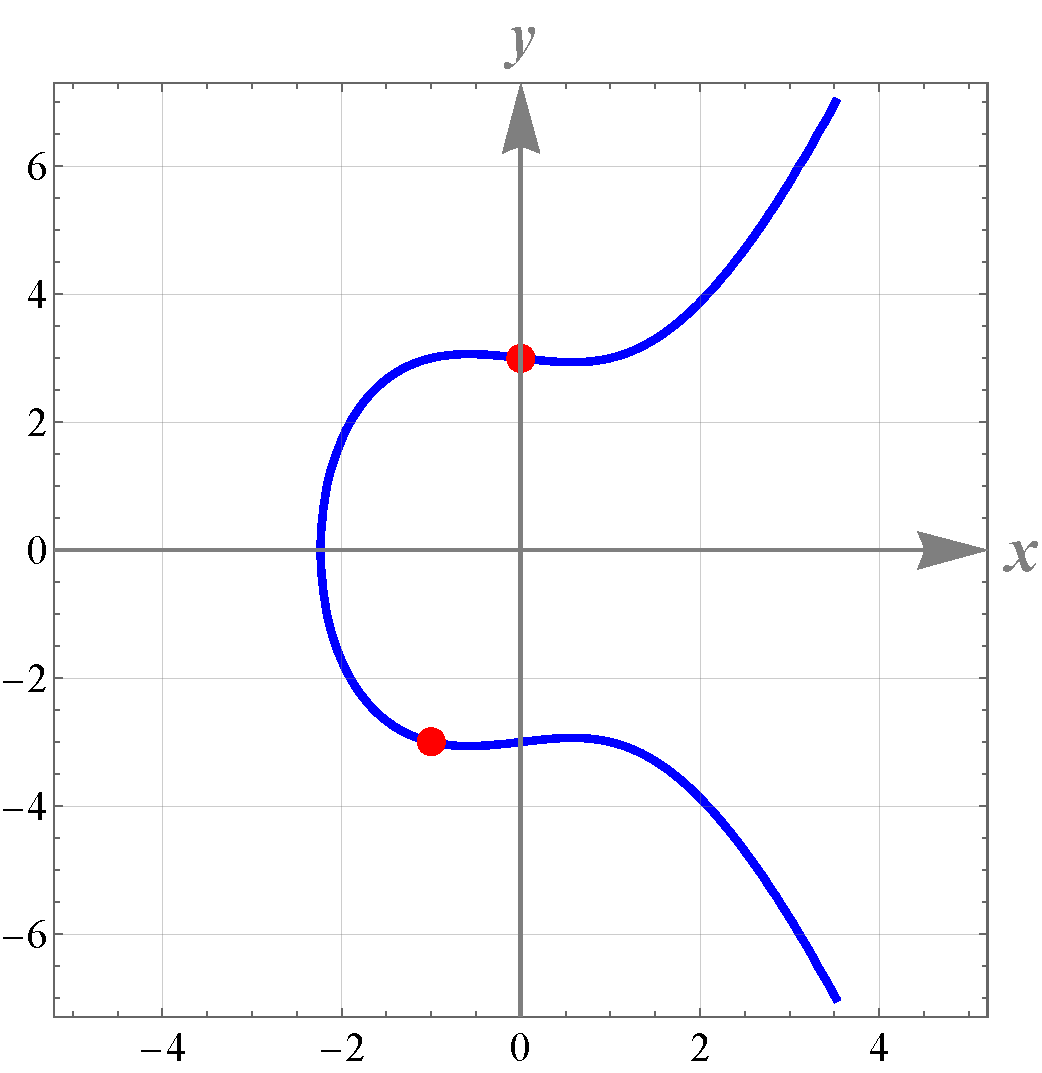
\includegraphics[width=0.4\textwidth]{images/lecture_3/ec_illustration_1.pdf}
                \label{fig:ec_1}
            \end{figure}
        \end{example}
    \end{frame}

    \begin{frame}{More Examples}
        Some more examples\footnote{Figure taken from ``Pairings for Beginners''}:
        \begin{figure}
            \centering
            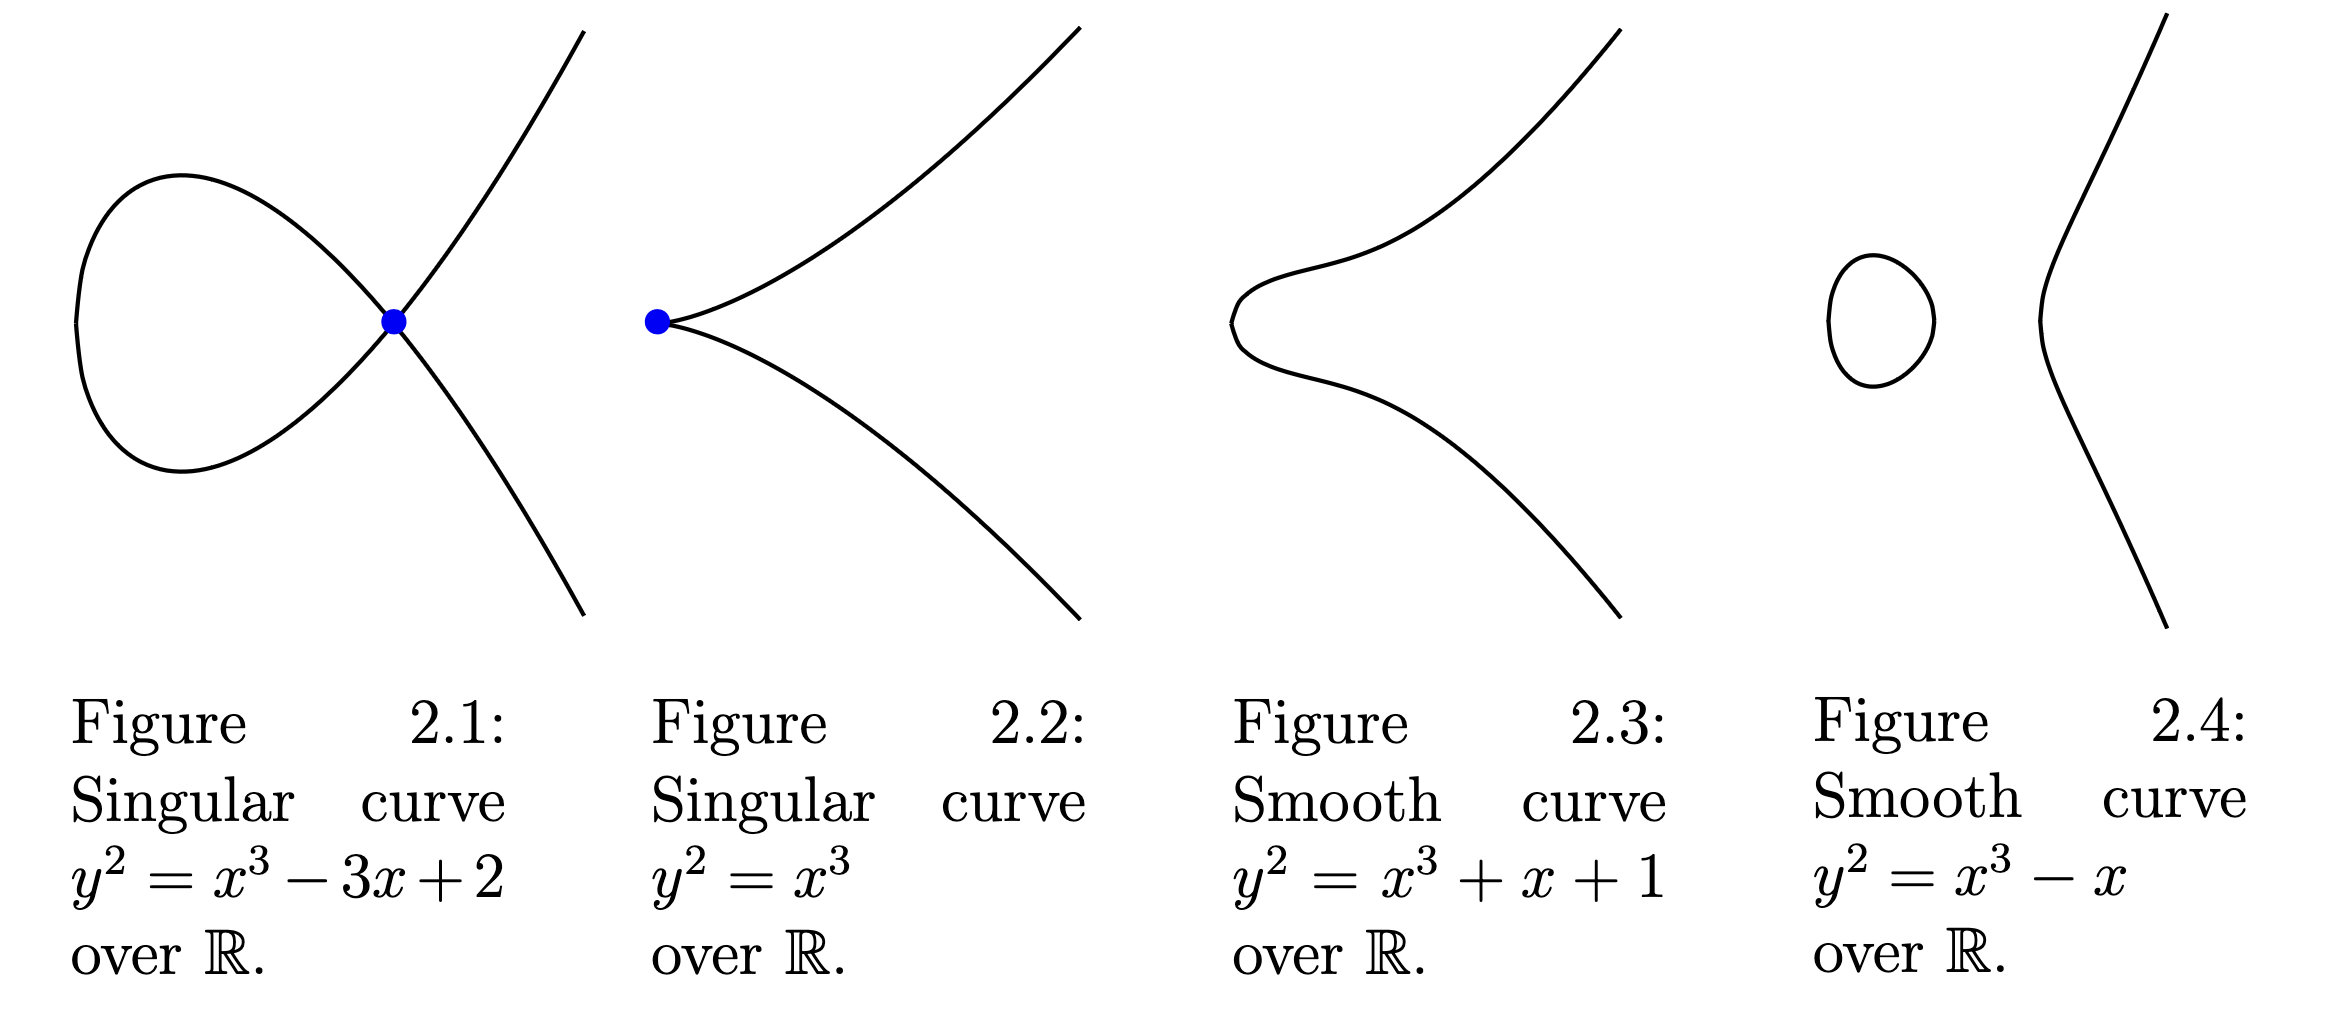
\includegraphics[width=\textwidth]{images/lecture_3/ec_illustration_2.png}
            \label{fig:ec_2}
        \end{figure}
    \end{frame}
    

    \begin{frame}{Real Elliptic Curves}
        But real elliptic curves are not that simple. Here how they look like\footnote{Figure taken from ``Moonmath''}:
        \begin{figure}
            \centering
            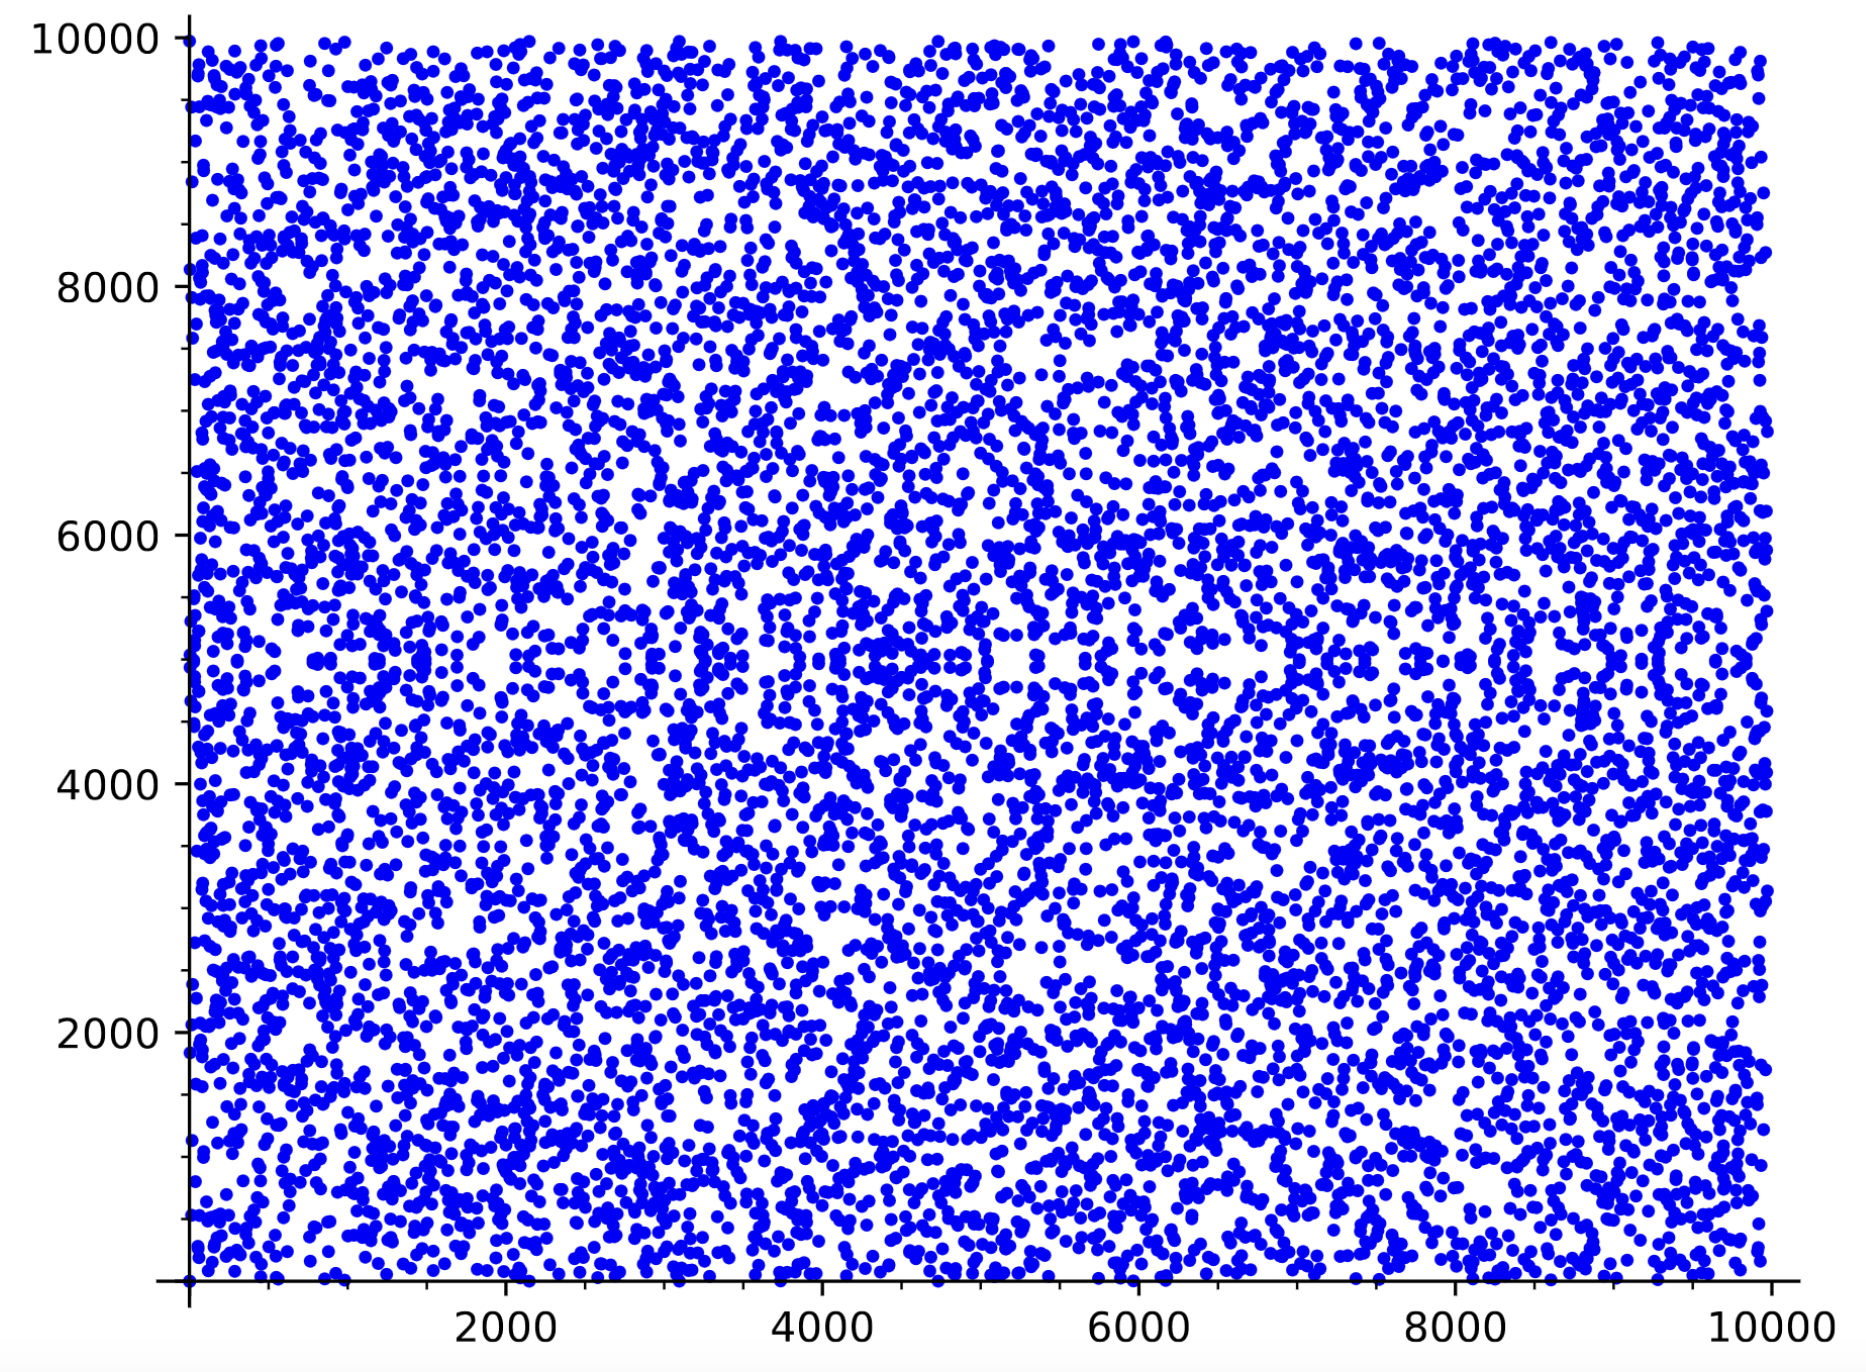
\includegraphics[width=0.6\textwidth]{images/lecture_3/ec_illustration_3.png}
            \caption{Curve $E/\mathbb{F}_{9973}: y^2 = x^3-2x+1$ over the finite field}
            \label{fig:ec_3}
        \end{figure}
    \end{frame}

    \subsection{Group Structure}

    \begin{frame}{Defining a Group Structure: A Few Words}
        \begin{definition}
            The set of points on the curve, denoted as $E_{a,b}(\mathbb{K})$, is defined as:
            \begin{equation*}
                E_{a,b}(\mathbb{K}) = \{(x,y) \in \mathbb{A}^2(\mathbb{K}): y^2=x^3+ax+b\} \cup \{\mathcal{O}\},
            \end{equation*}
            where $\mathcal{O}$ is the so-called \textbf{point at infinity}.
        \end{definition}

        \begin{block}{Remark \#1}
            If $(x_P,y_P) \in E(\mathbb{K})$ then $(x_P,-y_P) \in E(\mathbb{K})$.
        \end{block}

        \begin{block}{Remark \#2}
            Typically, $\mathbb{K} = \overline{\mathbb{F}}_p$: we do not conretize over which finite field we define the elliptic curve.
        \end{block}
    \end{frame}

    \begin{frame}{Defining a Group Structure: Chord Method}
        \begin{figure}
            \centering
            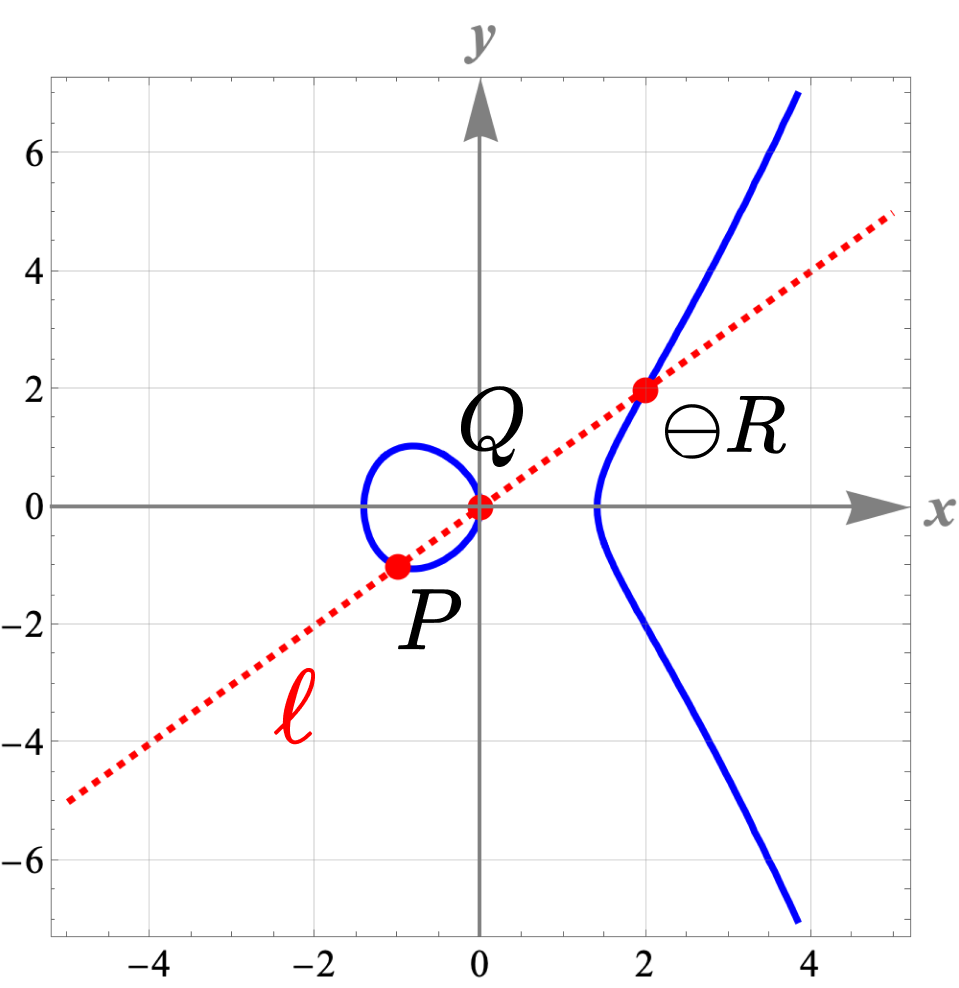
\includegraphics[width=0.525\textwidth]{images/lecture_3/ec_illustration_4.png}
            \caption{Chord method for adding two points}
            \label{fig:ec_4}
        \end{figure}
    \end{frame}

    \begin{frame}{Defining a Group Structure: Tangent Method}
        \begin{figure}
            \centering
            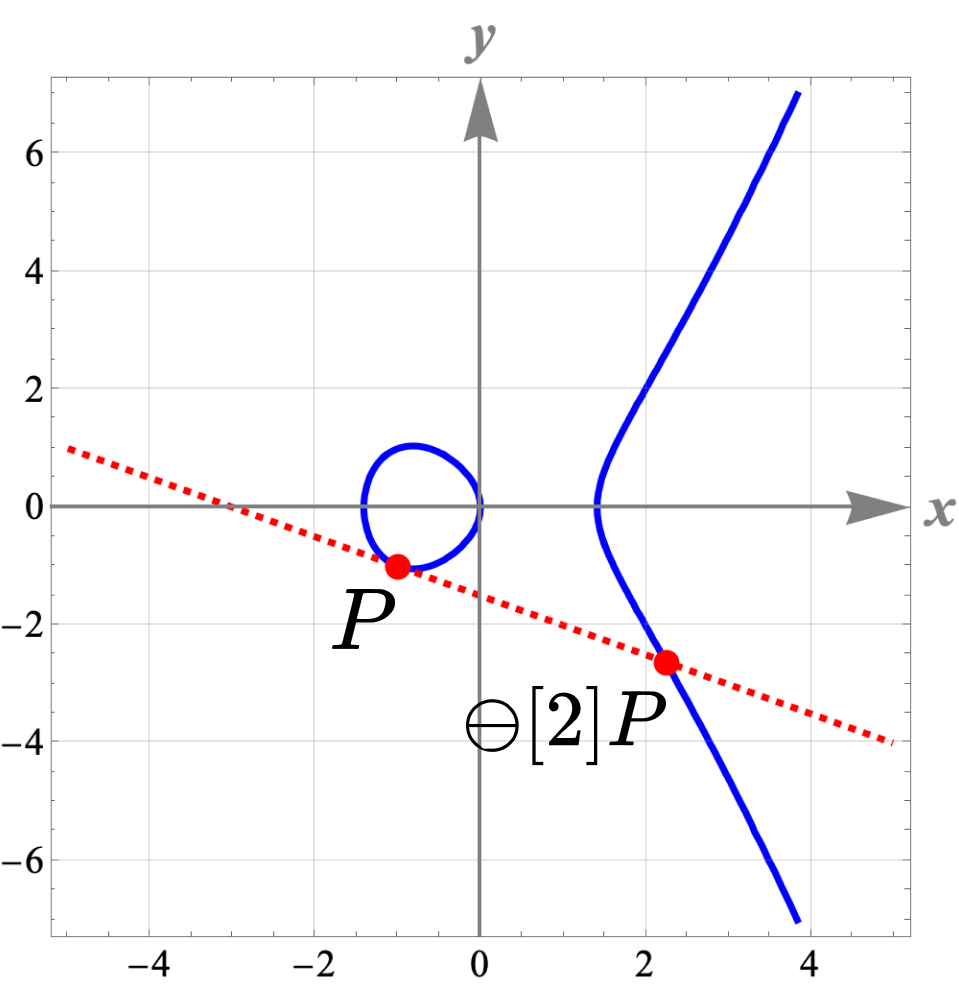
\includegraphics[width=0.525\textwidth]{images/lecture_3/ec_illustration_5.png}
            \caption{Tangent method for the point doubling}
            \label{fig:ec_5}
        \end{figure}
    \end{frame}

    \begin{frame}{Idea of Derivation}
        Line equation through $P=(x_P,y_P),Q=(x_Q,y_Q)$:
        \begin{equation*}
            \ell: y = \lambda (x-x_P) + y_P, \; \lambda = \frac{y_Q-y_P}{x_Q-x_P}
        \end{equation*}

        So all we need is to solve the system of equations:
        \begin{equation*}
            \begin{cases}
                y^2 = x^3+ax+b\\
                y = \lambda (x-x_P) + y_P
            \end{cases}
        \end{equation*}

        Substituting $y$ from the second equation to the first one, we get a cubic equation. Using Vieta's formula, one can derive
        \begin{equation*}
            x_P + x_Q + x_R = \lambda^2
        \end{equation*}

        The rest is easy to finish.
    \end{frame}

    \begin{frame}{Group Law}
        \begin{definition}
            \begin{enumerate}
                \item Point at infinity $\mathcal{O}$ is an identity element. 
                \item If $x_P\neq x_Q$, use the \textbf{chord method}. Define $\lambda := \frac{y_P-y_Q}{x_P-x_Q}$ --- the slope between $P$ and $Q$. Set the resultant coordinates as:
                \begin{equation*}
                    x_R := \lambda^2 - x_P - x_Q, \quad y_R := \lambda(x_P-x_R)-y_P.
                \end{equation*}
                \item If $x_P=x_Q$ and $y_P=y_Q$ (that is, $P=Q$), use the \textbf{tangent method}. Define the slope of the tangent at $P$ as $\lambda := \frac{3x_P^2+a}{2y_P}$ and set
                \begin{equation*}
                    x_R := \lambda^2 - 2x_P, \quad y_R := \lambda(x_P-x_R)-y_P.
                \end{equation*}
                \item Otherwise, define $P \oplus Q := \mathcal{O}$.
            \end{enumerate}
        \end{definition}
    \end{frame}

    \begin{frame}{One more Illustration}
        \begin{figure}[H]
            \centering
            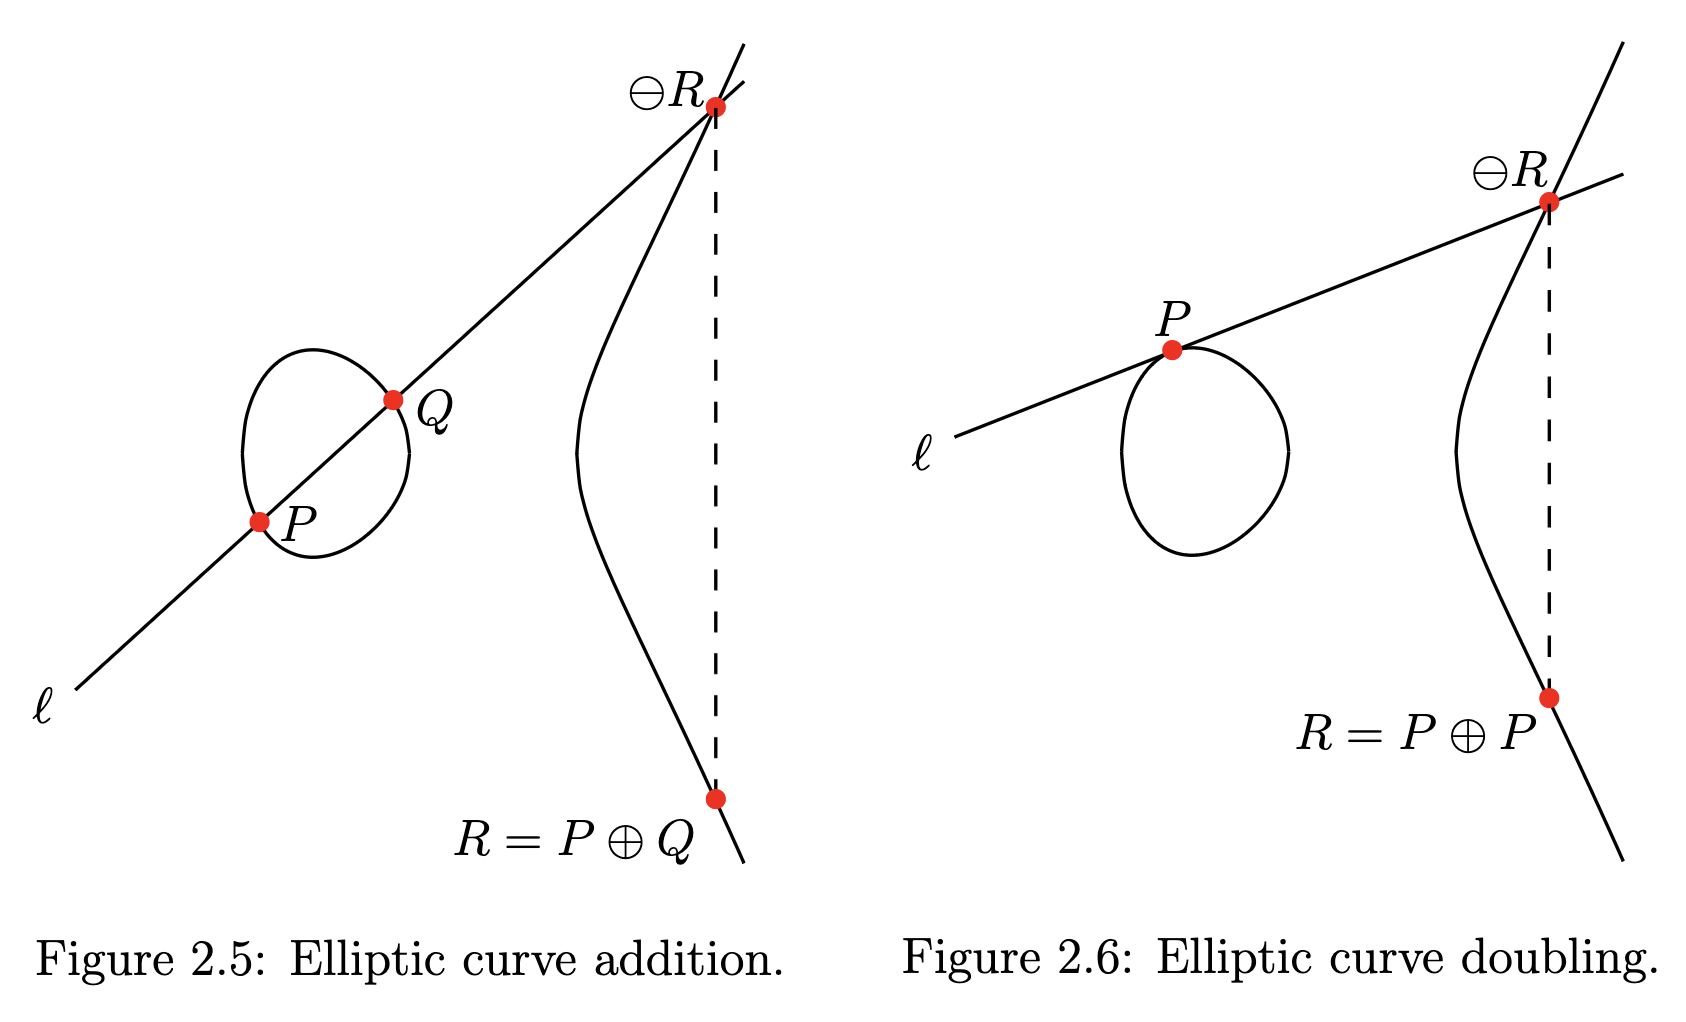
\includegraphics[width=\textwidth]{images/lecture_3/group_law.png}
            \label{fig:group_law}
        \end{figure}
    \end{frame}

    \begin{frame}{Example}
        \begin{example}
        Consider $E/\mathbb{R}: y^2=x^3-2x$. 
        \begin{itemize}
            \item \textbf{Addition:} $(-1,1) \oplus (0,0) = (2,-2), \; (2,2) \oplus (-1,-1) = (0,0)$.
            \item \textbf{Doubling:} $[2](-1,-1) = \left(\frac{9}{4},-\frac{21}{8}\right)$.
        \end{itemize}
        \begin{figure}
            \centering
            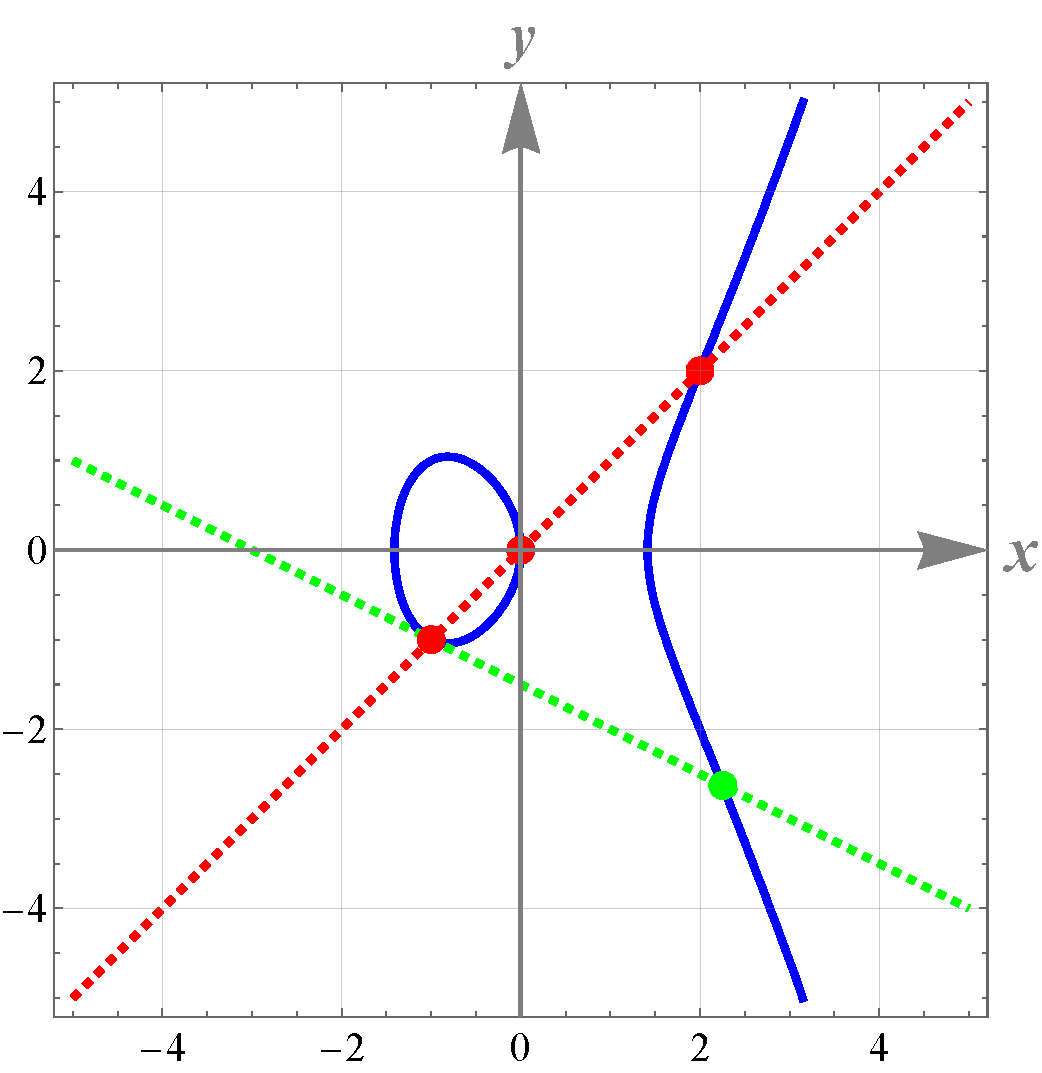
\includegraphics[width=0.35\textwidth]{images/lecture_3/ec_illustration_6.pdf}
            \label{fig:ec_6}
        \end{figure}
        \end{example}
    \end{frame}

    \begin{frame}{Hasse's Theorem}
        \begin{theorem}
            $(E(\overline{\mathbb{F}}),\oplus)$ forms an abelian group.
        \end{theorem}
        \vspace{10px}

        Now, let us consider the group order $r := |E(\mathbb{F}_{p^m})|$.

        \begin{theorem}
            \textbf{Hasse's Theorem on Elliptic Curves.} $r = p^m + 1 - t$ for some integer $|t| \leq 2\sqrt{p^m}$. A bit more intuitive explanation: the number of points on the curve is close to $p^m+1$. The value $t$ is called the \textbf{trace of Frobenius}.
        \end{theorem}
        
        \begin{block}{Remark}
            In fact, $r=|E(\mathbb{F}_{p^m})|$ can be computed in $O(\log(p^m))$, so the number of points can be computed efficiently even for fairly large primes $p$.
        \end{block}
    \end{frame}

    \begin{frame}{Discrete Logarithm}
        \begin{definition}
           
            Let $P \in E(\overline{\mathbb{F}}_p)$ and $\alpha \in \mathbb{Z}_r$. Define the scalar multiplication $[\alpha]P$ as adding $P$ to itself $\alpha-1$ times (also set $[0]P := \mathcal{O}$).
            
        \end{definition}

        \begin{definition}
            Suppose $E$ is cyclic, meaning, $\langle G \rangle = E$ for some $G \in E$. The \textbf{discrete logarithm problem} on $E$ consists in the following: suppose $P = [\alpha]G$ for some $\alpha \in \mathbb{Z}_r$. Find $\alpha$ based on $P$.
        \end{definition}

        \begin{block}{Remark}
            If $r$ is a product of primes $p_1,p_2,\dots,p_k$ such that $p_1<p_2<\dots< p_k$, then the best-known algorithm to solve the discrete logarithm problem is no significantly better than $O(\sqrt{p_1})$.
        \end{block}
    \end{frame}

    \begin{frame}[plain, standout]
        \centering
        \LARGE
        \textbf{Thank you for your attention} \\
        
        \vspace{0.2cm} \Huge \ding{170} \large \\
        
        \vspace{1cm}
  
        \href{https://zkdl-camp.github.io/}{\raisebox{-.1em}{\hspace{.025em}\faIcon{globe}}\hspace{.325em}zkdl-camp.github.io} \\
  
        \href{https://github.com/ZKDL-Camp}{\raisebox{-.1em}{\hspace{.025em}\faIcon{github}}\hspace{.325em}github.com/ZKDL-Camp}
        
        \begin{center}
            
\includegraphics[width=0.15\textwidth]{images/logo.png}
        \end{center}
    \end{frame}
\end{document}